\documentclass[10pt]{exam}

\usepackage[margin=1in]{geometry}
\usepackage{amsmath}
\usepackage{amssymb}
\usepackage{amsthm}
\usepackage{mathtools}
\usepackage{bm}
\usepackage{stmaryrd}
\usepackage{booktabs}

\usepackage{color}
\usepackage{colortbl}
\definecolor{deepblue}{rgb}{0,0,0.5}
\definecolor{deepred}{rgb}{0.6,0,0}
\definecolor{deepgreen}{rgb}{0,0.5,0}
\definecolor{gray}{rgb}{0.7,0.7,0.7}

\usepackage{hyperref}
\hypersetup{
  colorlinks   = true, %Colours links instead of ugly boxes
  urlcolor     = black, %Colour for external hyperlinks
  linkcolor    = blue, %Colour of internal links
  citecolor    = blue  %Colour of citations
}

\usepackage{listings}

%%%%%%%%%%%%%%%%%%%%%%%%%%%%%%%%%%%%%%%%%%%%%%%%%%%%%%%%%%%%%%%%%%%%%%%%%%%%%%%%

\theoremstyle{definition}
\newtheorem{problem}{Problem}
\newtheorem{example}{Example}
\newtheorem{note}{Note}
\newtheorem{defn}{Definition}
\newtheorem{fact}{Fact}
\newtheorem{refr}{References}
\newtheorem{theorem}{Theorem}
\newcommand{\E}{\mathbb E}
\newcommand{\R}{\mathbb R}
\DeclareMathOperator{\nnz}{nnz}
\DeclareMathOperator{\sign}{sign}
\DeclareMathOperator{\determinant}{det}
\DeclareMathOperator{\Var}{Var}
\DeclareMathOperator{\rank}{rank}
\DeclareMathOperator{\prob}{\mathbb P}
\DeclareMathOperator*{\argmin}{arg\,min}
\DeclareMathOperator*{\argmax}{arg\,max}

\newcommand{\Ein}{E_{\text{in}}}
\newcommand{\Eout}{E_{\text{out}}}
\newcommand{\Etest}{E_{\text{test}}}
\newcommand{\I}{\mathbf I}
\newcommand{\Q}{\mathbf Q}
\newcommand{\p}{\mathbf P}
\newcommand{\pb}{\bar {\p}}
\newcommand{\pbb}{\bar {\pb}}
\newcommand{\pr}{\bm \pi}

\newcommand{\trans}[1]{{#1}^{T}}
\newcommand{\loss}{\ell}
\newcommand{\w}{\mathbf w}
\newcommand{\wstar}{{\w}^{*}}
\newcommand{\x}{\mathbf x}
\newcommand{\y}{\mathbf y}
\newcommand{\lone}[1]{{\lVert {#1} \rVert}_1}
\newcommand{\ltwo}[1]{{\lVert {#1} \rVert}_2}
\newcommand{\lp}[1]{{\lVert {#1} \rVert}_p}
\newcommand{\linf}[1]{{\lVert {#1} \rVert}_\infty}
\newcommand{\lF}[1]{{\lVert {#1} \rVert}_F}

\newcommand{\mH}{m_{\mathcal H}}
\newcommand{\dvc}{{d_{\text{VC}}}}
\newcommand{\HH}[1]{\mathcal H_{\text{#1}}}
\newcommand{\Hbinary}{\HH_{\text{binary}}}
\newcommand{\Haxis}{\HH_{\text{axis}}}
\newcommand{\Hperceptron}{\HH_{\text{perceptron}}}


\newcommand{\ignore}[1]{}

%%%%%%%%%%%%%%%%%%%%%%%%%%%%%%%%%%%%%%%%%%%%%%%%%%%%%%%%%%%%%%%%%%%%%%%%%%%%%%%%

\begin{document}


\begin{center}
{
\Huge
Chapter 3.4: Non-linear Transformations
}
\end{center}

\section*{Overview}

In this section, we will see how to build non-linear models out of linear models.
This will allow us to easily construct models with different VC dimensions that are appropriate for our datasets.

\vspace{0.15in}
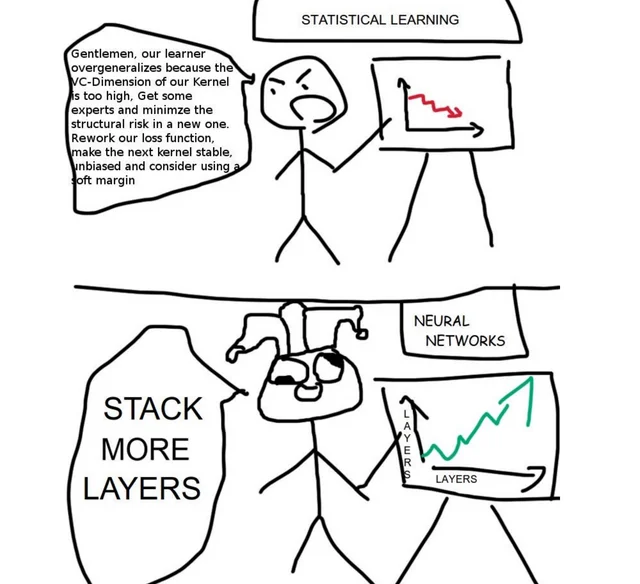
\includegraphics[width=3in]{layers}

\vspace{0.15in}
\begin{defn}
    Define a \emph{feature transform} as it relates to the perceptron hypothesis class.
\end{defn}
\ignore{
Recall that the perceptron hypothesis class is defined to be
\begin{equation}
    \HH{} = \bigg\{ \x \to \sign(\trans\w\x) : \w \in \R^d \bigg\},
\end{equation}
and it has VC dimension $\Theta(d)$, which controls the generalization error.
Feature transforms are one of our primary tools for generating new hypothesis classes with different statistical properties.
%A feature map is a function $\Phi : d \to 	\tilde d$
%Feature transforms are a tool for manipulating the VC dimension of a hypothesis class.
%\begin{defn}
    \begin{defn}
    A \emph{feature transform} (or \emph{feature map}) is a function $\Phi : \R^d \to \R^{	\tilde d}$ that we apply to our data points before passing them to our model.
        We call the domain of $\Phi$ (i.e.\ $\R^d$) the \emph{original data space} and the range of $\Phi$ (i.e.\ $\R^{	\tilde d}$) the \emph{feature space}.
    \end{defn}
    \begin{note}
        A \emph{kernel} is a type of function closely related to feature transforms that are used for speeding up certain types of calculations.
        There exists a bijection between kernel functions and feature transforms,
        and so people often use these terms interchangeably.
    \end{note}
    We can use these feature transforms to create new hypothesis classes based on the perceptron hypothesis class:
\begin{equation}
    \HH{$\Phi$} = \bigg\{ \x \to \sign(\trans\w\Phi(\x)) : \w \in \R^{	\tilde d} \bigg\}.
\end{equation}
Our choice of feature transform will have a profound impact on the statistical properties of the resulting hypothesis class.

%\vspace{6in}
\begin{note}
    Feature maps with the perceptron hypothesis class are state-of-the-art for MANY applications.
    Essentially, deep learning is best for vision (always), text (sometimes), and feature maps are the best for everything else.
\end{note}
    }

\newpage
\section*{Generic Feature Transforms}

\begin{problem}
    The \emph{polynomial feature map} is a generalization of the examples above.
    It is one of the most popular feature maps due to its simplicity,
    and it is the main example in the textbook (see pages 99-104).

    The polynomial map of degree $Q$ (denoted $\Phi_Q$ in the book) has one feature for each of the $Q$ degree monomials formed by the input data dimensions.
    For example, in 2 dimensions, the 2nd degree polynomial feature map is
    \begin{equation}
        \Phi_2(\x) = (x_1, x_2, x_1^2, x_2^2, x_1x_2)
    \end{equation}
    and the 3rd degree polynomial feature map is
    \begin{equation}
        \Phi_3(\x) = (x_1, x_2, x_1^2, x_2^2, x_1x_2, x_1^3, x_2^3, x_1^2x_2, x_1x_2^2)
        .
    \end{equation}
            %Explain this phenomenon in terms of VC theory.

    \begin{enumerate}
        \item
            How does the choice of $Q$ affect $\Ein$?
            \vspace{6in}

        The following two links visualize this transformation.
        The first link is closely related to the examples in Figures 3.5 and 3.6;
            the second link is an entirely separate example.
        \begin{enumerate}
            \item \url{https://www.youtube.com/watch?v=3liCbRZPrZA}
                %\vspace{2in}
                %\newpage
            \item \url{https://www.youtube.com/watch?v=ndNE8he7Nnk}
                %\vspace{2in}
        \end{enumerate}

        \item
            What is the \emph{universal approximation property}?
            \vspace{3in}

            \newpage
        \item
        The VC dimension of the hypothesis space $\HH{$\Phi$}$ equals $	\tilde d$.
        What is a formula for $	\tilde d$ (and thus the VC dimension) based on $Q$ and $d$?
            \vspace{4in}

        % (Q + d \choose d) - 1

        \item
        When would we want to use the polynomial kernel?
    \end{enumerate}
\end{problem}

%\begin{problem}
    %The gaussian feature map is defined as
%\end{problem}

%\section*{Dimensionality Reduction}
%

\newpage
\begin{problem}
    The PCA feature map is an example of a \emph{dimensionality reduction} technique.
    It is defined to be
    \begin{equation}
        \Phi(\x) = \trans\x A
    \end{equation}
    where $A$ is a $d\times 	\tilde d$ matrix with the $i$th column equal to the $i$th eigenvector of $\trans X X$,
    and $X : N \times d$ is the matrix of all data vectors.
    The $A$ matrix is constructed this way because this selects a subspace with ``maximum variance''.

    NOTE:
    For a cool example with ``eigenfaces'', see the scikit-learn documentation:
    \url{https://scikit-learn.org/stable/auto_examples/applications/plot_face_recognition.html}.
    
    NOTE: Most explanations of PCA focus on why this choice of matrix maximizes the variance and ignore the statistical properties of classifiers created with PCA features.
    What actually matters in practice are these statistical properties, and so that's what we'll focus on here.
    Sometimes, machine learning technical interviewers will ask about why the eigenvalues maximize the variance, and so while you don't need to know that for this class (and it is not covered in the textbook), it is worth reviewing before interviewing.
    For an explanation, see stackoverflow: \url{https://stats.stackexchange.com/a/140579/16243}.

    \begin{enumerate}
    \item How does $\tilde d$ affect $\Ein$?
        \vspace{3in}
    \item How does $\tilde d$ affect the VC dimension (and thus the generalization error)?
        \vspace{3in}
    \end{enumerate}
\end{problem}

\section*{Popular Models as ``Just'' Feature Maps}

\begin{problem}
    The random feature map is defined as 
    \begin{equation}
        \Phi(\x) = \trans\x A
    \end{equation}
    where $A$ is a random $d\times 	\tilde d$ matrix.
    Any distribution can be used to select the entries of the $A$ matrix, but some common choices are the uniform distribution over $(-1,1)$ or the standard gaussian distribution with mean 0 and variance 1.

    The hypothesis class $\HH{$\Phi$}$ (i.e.\ random features with the perceptron hypothesis class) is often called the \emph{random kitchen sink}.
    It was first introduced in 2006, and in 2017 it received the ``Test of Time'' award at the NIPS conference (now called NeurIPS).
    This random kitchen sink won this award because it remains state-of-the-art for MANY applications.
    You can watch the award presentation at \url{https://www.youtube.com/watch?v=ORHFOnaEzPc}. % &t=10m23s

    \begin{enumerate}
        \item
            How does $\Ein$ vary with $	\tilde d$?
            \vspace{3in}

        \item
            How does $\Ein$ for random features compare to the $\Ein$ for PCA?
            \vspace{3in}

            \newpage
        \item
            What is the VC dimension if $	\tilde d \le d$?
            \vspace{4in}

        \item
            What is the VC dimension if $	\tilde d > d$?
            \vspace{3in}

            \newpage
        \item
            Under what conditions would you want to use the random feature map or PCA?
    \end{enumerate}
\end{problem}

\newpage
\begin{problem}
    (See Example 3.15 in the textbook.)
    Define the feature map
    \begin{equation}
        \Phi_{(k)}(\x) = (1, x_k)
    \end{equation}
    to extract the $k$th coordinate from the input data point and let $\HH{$\Phi_{(k)}$}$ be the hypothesis class of perceptrons with the above feature map.
    The \emph{decision stump} hypothesis class is defined to be
    \begin{equation}
        \HH{stump} = \cup_{k=1}^d \HH{$\Phi_{(k)}$}.
    \end{equation}
    \begin{enumerate}
        \item
            State an upper bound on the VC dimension of $\HH{stump}$ in terms of $d$ using big-O notation.
            (Hint: This bound is given in the textbook in a form that doesn't use big-O notation.)
            \vspace{3in}
        \item
            The decision stump is a popular model for datasets with many dimensions but few data points.  Explain why using VC theory.
            \vspace{3in}
    \end{enumerate}
\end{problem}

\newpage
\section*{Single Feature Transformations}

\begin{problem}
    Many features are ``discrete''.
    That is, they have a fixed number of values where the value has little semantic meaning.
    For example, marital status in the famous German Credit dataset\footnote{\url{http://archive.ics.uci.edu/dataset/144/statlog+german+credit+data}} is encoded as a column with the following semantics:

    \vspace{0.15in}
    \begin{tabular}{ll}
        \toprule
        column value & semantic meaning \\
        \midrule
        1 & single - never married \\
        2 & married - first marriage \\
        3 & single - divorced \\
        4 & single - widowed \\
        5 & married - remarried (female) \\ 
        6 & married - remarried (male) \\ 
        \bottomrule
    \end{tabular}

    \vspace{0.15in}
    \noindent
    The \emph{one-hot encoding} converts these discrete columns into multiple boolean columns, one for each value in the original column.
    The one-hot encoding for marital status above would convert a single column into 5 separate columns in the feature space.
    This conversion often greatly improves $\Ein$ because a linear separation of the original discrete values often has no semantic meaning.
    \begin{enumerate}
        \item 
            If the discrete column has $c$ possible values,
            then the feature space has $	\tilde d = d + c - 1$ columns.
            What is the VC dimension of $\HH{$\Phi$}$?
            \vspace{1.5in}

        \item
            The number of discrete values can sometimes be extremely large.
            For example, $c$ might be the city that a person was born in, and there are millions of cities in the world.
            \begin{enumerate}
            \item From a VC perspective, why is this a problem?
                \vspace{1.5in}
            \item How can we fix this problem?
            \end{enumerate}
    \end{enumerate}
\end{problem}

%\begin{problem}
    %Many types of features are ``cyclic''.
    %A common example is the time of day that an event happened.
    %This is commonly encoded as the number of seconds that have elapsed since midnight.
    %Events that happen near midnight cannot be well classified with a linear model when represented this way.
%
    %The $k$-way sin transform
%\end{problem}

\newpage
\section*{Other Operations}

\begin{problem}
    The \emph{mean centering} feature transformation is defined to be
    \begin{equation}
        \Phi(\x) = \x - \mu,
    \end{equation}
    where
    \begin{equation}
        \mu = \frac 1 N \sum_{i=1}^N \x_i.
    \end{equation}
    \begin{enumerate}
        \item What is the VC dimension of $\HH{$\Phi$}$?
            \vspace{3in}
        \item When should you use the mean centering feature transformation?
            \vspace{2in}
    \end{enumerate}
\end{problem}

\newpage
\begin{problem}
    The \emph{range normalization} feature transformation rescales all of the features to between $[-1, 1]$.
    It is defined to be
    \begin{equation}
        \phi(\x)_i = x_i/\alpha_i
    \end{equation}
    where $\alpha_i$ is the maximum absolute value of the $x_i$ component of all the training datapoints.

    NOTE: The lowercase $\phi$ instead of the uppercase $\Phi$ above is intentional.
    It is the book's notation to let you know that the index refers to a specific column of the output of the $\Phi$ function.
    \begin{enumerate}
        \item What is the VC dimension of $\HH{$\Phi$}$?
            \vspace{3in}
        \item When should you use the range normalization transformation?
            \vspace{3in}
    \end{enumerate}
\end{problem}

\end{document}



